% This voodoo is needed for arXiv scripts and must appear within the first 4 lines
\pdfoutput=1
\documentclass[aps,prd,amsmath,floats,floatfix, twocolumn,
superscriptaddress,nofootinbib,showpacs]{revtex4-1}

% UTF8 always
\usepackage[T1]{fontenc}
\usepackage[utf8]{inputenc}
\usepackage{lmodern}
\usepackage{verbatim}

\usepackage[dvipsnames, usenames]{xcolor}
\definecolor{linkcolor}{rgb}{0.0,0.3,0.5}
\usepackage[hypertexnames=false, unicode, colorlinks=true, linkcolor=linkcolor,
citecolor=linkcolor, filecolor=linkcolor,urlcolor=linkcolor,
pdfusetitle]{hyperref}

%\usepackage[colorlinks, pdfborder={0 0 0}, plainpages=false]{hyperref}
\usepackage[all]{hypcap}
\usepackage{graphicx}
\usepackage{xspace}
%\usepackage[usenames,dvipsnames]{color}
\usepackage{amssymb}
% \usepackage[normalem]{ulem} %for \sout
\usepackage{bm} % boldmath

% Better spacing
\usepackage{microtype}

\usepackage[english]{babel}
% \usepackage{blindtext}

%
\graphicspath{%
  {figs/}%
  % More directories are added in braces, without commas between
}


\DeclareMathAlphabet{\mathpzc}{OT1}{pzc}{m}{it}

\newcommand{\roughly}{\mathchar"5218\relax\,} % Different from \sim in spacing
\newcommand{\into}{\!\times\!\relax} % Different from \times in spacing

% Macros for text changes
\newcommand{\red}{\textcolor{red}}
\newcommand{\vv}[1]{\textcolor{WildStrawberry}{VV: #1}}

\newcommand{\Note}[1]{\textcolor{blue}{\textbf{[#1]}}}
\newcommand{\h}{\mathpzc{h}}
\newcommand{\hlm}{\mathpzc{h}_{\ell m}}
\newcommand{\chieff}{\chi_{\mathrm{eff}}}
\newcommand{\chiPN}{\chi_{\mathrm{PN}}}


\newcommand{\bfemph}[1]{\emph{\textbf{#1}}}

\newcommand{\nn}{\nonumber}

\newcommand{\cd}{\nabla}
\newcommand{\pd}{\partial}
\newcommand{\lie}{\mathcal{L}}
\newcommand{\dd}{\mathrm{d}}

\newcommand{\TODO}[1]{\red{TODO: #1}}
\newcommand{\AddCite}{\red{[Needs citation]}}

\newcommand{\avgOmega}{\omega^{\text{avg}}_{22}}
\newcommand{\eEOB}{e_{\text{EOB}}}
\newcommand{\zeroA}{A_{22}^{e=0}}
\newcommand{\zeroOmega}{\omega_{22}^{e=0}}
\newcommand{\tref}{t_{\text{ref}}}
\newcommand{\fref}{f_{\text{ref}}}
\newcommand{\mAmp}{\texttt{Amplitude}}
\newcommand{\mFreq}{\texttt{Frequency}}
\newcommand{\mResAmp}{\texttt{ResidualAmplitude}}
\newcommand{\mResFreq}{\texttt{ResidualFrequency}}
\newcommand{\mFreqFits}{\texttt{FrequencyFits}}
\newcommand{\resAmp}{\Delta A_{22}}
\newcommand{\resOmega}{\Delta \omega_{22}}

% \newcommand{\mat}{{\tiny{\mathrm{mat}}}}
% \newcommand{\mat}{{(\mathrm{m})}}
\newcommand{\txt}[1]{{\textrm{\tiny{#1}}}}

%%%%%%%%%%%%%%%%%%%%%%%%%%%%%%%%%%%%%%%%%%%%%%%%%%%%%%%%%%%%%%%%%%%%%%%%%%%
\begin{document}

\title{Defining eccentricity for gravitational wave astronomy}

\newcommand{\Cornell}{\affiliation{Cornell Center for Astrophysics
    and Planetary Science, Cornell University, Ithaca, New York 14853, USA}}
\newcommand\CornellPhys{\affiliation{Department of Physics, Cornell
    University, Ithaca, New York 14853, USA}}
\newcommand\Caltech{\affiliation{TAPIR 350-17, California Institute of
    Technology, 1200 E California Boulevard, Pasadena, CA 91125, USA}}
\newcommand{\AEI}{\affiliation{Max Planck Institute for Gravitational Physics
    (Albert Einstein Institute), Am M\"uhlenberg 1, Potsdam 14476, Germany}} %
\newcommand{\UMassD}{\affiliation{Department of Mathematics,
    Center for Scientific Computing and Visualization Research,
    University of Massachusetts, Dartmouth, MA 02747, USA}}
\newcommand\Olemiss{\affiliation{Department of Physics and Astronomy,
    The University of Mississippi, University, MS 38677, USA}}
\newcommand{\Bham}{\affiliation{School of Physics and Astronomy and Institute
    for Gravitational Wave Astronomy, University of Birmingham, Birmingham, B15
    2TT, UK}}
\newcommand{\ICTS}{\affiliation{International Centre for Theoretical Sciences,
    Tata Institute of Fundamental Research, Bangalore 560089, India}}


\author{Md Arif Shaikh}
\email{arif.shaikh@icts.res.in}
\ICTS

\author{Vijay Varma}
\email{vijay.varma@aei.mpg.de}
\thanks{Marie Curie Fellow}
\AEI

\author{Antoni Ramos-Buades}
\AEI

\author{Harald P. Pfeiffer}
\AEI

\author{Maarten van de Meent}
\AEI

% Because hyperref only gets the *last* author, we need to be explicit.
\hypersetup{pdfauthor={Varma et al.}}

\date{\today}

%==========================================================================
\begin{abstract}
Eccentric Compact Binary Coalescences (CBCs) are important science
targets of Gravitational Wave (GW) observatories.  Many different
eccentricity definitions exist in the literature.  This paper
continues the development of a definition of eccentricity that is
defined based solely on the gauge invariant gravitational waveforms
and applicable to gravitational waveforms of many origins. Our
proposal improves on related works in that the new definition agrees
in the Newtonian limit with the standard Newtonian definition of
eccentricity. We present a public implementation of the proposed
algorithm and demonstrate its robustness on waveforms of various
origin, ranging from quasi-circular to highly eccentric systems.  The
present work focuses on aligned-spin binaries which do not exhibit
orbital precession. Possible extensions to precessing binaries are
discussed.
\end{abstract}

\maketitle

%==========================================================================
\section{Introduction}
\label{sec:introduction}
I done did it. Some other people that done'd similar things:
\cite{Scott:2015rza}.

%==========================================================================
\section{Definig eccentricity and mean anomaly}
\label{sec:defining-eccentricity-and-mean-anomaly}
We propose a definition of eccentricity inspired by previous works in
the literature (\TODO{cite papers}) using the frequency of the (2, 2)
mode of gravitational wave at the pericenter (point of nearest
approach) and the apocenter (point of largest separation), denoted
simply by $\omega_{p}$ and $\omega_{a}$, respectively.

\begin{equation}
\label{eq:eccentricity_definition} e(t) = \frac{\sqrt{\omega_{p}(t)} -
\sqrt{\omega_{a}(t)}}{\sqrt{\omega_{p}(t)} + \sqrt{\omega_{a}(t)}}
\end{equation}

This definition of eccentricity has the following features,
\begin{itemize}
\item It is a gauge indipendent definition of eccentricity that relies
only of gravitational wave data and therefore independent the model
that was used to generate the waveform in the first place.
\item It reduces to the well known Newtonian definition of
eccentricity in the Newtonian limit.
\item It smoothly goes to zero as the binary inspirals towards the
merger and lose eccentricity and becomes quasi-circular.
\end{itemize}

For an eccentric orbit, apart from the eccentricity, one can define
another quantity called the mean anomaly $l(t)$. In the Newtonian
context it is defined as
\begin{equation}
\label{eq:mean_anomaly_definition} l(t) = 2\pi \frac{t - t_0}{P}
\end{equation} where $t_0$ is the time of the last pericenter passage
and $P$ is the radial period which is defined to be the time between
two successive pericenter passages.  In the Newtonian case, the radial
period $P$ is a constant but in general relativistic case, it changes
as the binary inspirals.

In gravitational wave literature, the two gravitational wave
polarizations $\h_{+}$ and $\h_{\into}$ are conventionally presented
in the form of a complex function of time $\h(t) = \h_{+}(t) - i
\h_{\into}(t)$ which can be decomposed in terms of spin weighted
spherical harmonics of spin $-2$ denoted as ${}_{-2}Y_{\ell m}(\theta,
\varphi)$ and a complex gravitational wave mode $\hlm(t)$
\begin{equation}
  \label{eq:h} \h(t) \equiv \h_{+}(t) -i \h_{\into}(t) =
\sum_{\ell=2}^{\ell=\infty}\sum_{m=-\ell}^{m=\ell} {}_{-2}Y_{\ell
m}(\theta, \varphi) \hlm(t)
\end{equation} In the current work, the waveform modes at future null
infinity, scaled to unit mass and unit distance, is denoted as $\hlm$.

The $\hlm$ of the $(\ell, m)$ mode could be further decomposed in an
amplitude $A_{\ell m}$ and a phase $\phi_{\ell m}$ as
\begin{equation}
  \label{eq:amp-phase}
  \hlm(t) = A_{\ell m}(t) e^{i \phi_{\ell m}(t)}
\end{equation}
The frequency of $(2, 2)$ mode, therefore, could be obtained as
\begin{equation}
  \label{eq:omega22}
  \omega_{22}(t) = \frac{\dd \phi_{22}(t)}{\dd t}.
\end{equation}

Given a gravitational waveform, we proceed to measure the eccentricity
and mean anomaly using the eccentricity definition in
eq. (\ref{eq:eccentricity_definition}) and the mean anomaly definition
in eq. (\ref{eq:mean_anomaly_definition}), respectively, at the
desired reference time (or reference frequency) using the following
three steps

\begin{enumerate}
\item {\itshape Find the positions of the pericenter (local maxima)
and apocenter (local minima)} and get the values of $\omega_{22}$ at
the pericenter ($\omega_p$) and apocenter ($\omega_a$). There are
several ways to do this. However, not all of these different ways are
equally efficient in finding the local maxima and minima.  As the
eccentricity becomes smaller and smaller, some of these methods are
more efficient in finding the local maxima and minima than the
others. Once we find the locations of the maxima and the minima, we
evaluate the value of $\omega_{22}$ at these locations which give us
the $\omega_p$ and $\omega_a$ we need for the second step in
eccentricity measurement. In sec. \ref{sec:implementation}, we discuss
these different methods that have been implemented in our public
\texttt{Python} library to measure eccentricity.
\item {\itshape Construct interpolants $\omega_p(t)$ and
$\omega_a(t)$} using the values of $\omega_{22}$ at the pericenter and
apocenter, respectively, from the previous step.
\item Plug in the interpolants $\omega_p(t)$ and $\omega_a(t)$ in
(\ref{eq:eccentricity_definition}) to measure eccentricity. For mean
anomaly, use the positions of pericenter from the first step to find
the times of passage of pericenters and use those in
eq. (\ref{eq:mean_anomaly_definition}).
\end{enumerate}

In fig. \ref{fig:ecc_definition}, we illustrate how the measurements
of eccentricity and mean anomaly are done for a gravitational wave
from a numerical relatively simulation. Lower left panel shows the
instantaneous (2, 2) mode frequency $\omega_{22}(t)$ (light brown),
the positions of pericenters (violet circles) and apocenters (cyan
circles) and the interpolants $\omega_p(t)$ (violet solid line) and
$\omega_a(t)$ (cyan solid line). The upper left panel shows the
evolution of measured eccentricity $e(t)$.

Lower right panel shows the the $A_{22}(t)$ (solid line) and times of
passage of pericenters using the vertical dotted (green) lines. The
upper right panel shows the evolution of the mean anomaly
$l(t)$. Between two successive pericenters, the mean anomaly varies
linearly with time. The slope of the mean anomaly curves becomes
steeper as the binary inspirals towards merger due to decreasing
radial period $P_{i} = t_{i+1} - t_i$, where $t_{i}$ and $t_{i+1}$ are
the time of passages of $i$th and the $i+1$th pericenter, respectively
and $P_i$ is the radial period of the $i$th orbit.

The vertical dashed red lines in all the panels indicate the reference
time $\tref$ where we measure the eccentricity and mean
anomaly and the red circles on the upper left and upper right panels
represent the measured eccentricity and the measured mean anomaly,
respectively, at the reference time.

Instead of measuring eccentricity and mean anomaly at a reference
time, one may be interested in doing the measurement at a reference
frequency (\TODO{motivate why we want to measure at reference
frequency?}). However, for eccentric systems, the instantaneous
$\omega_{22}(t)$ is not a monotonic function of time. Therefore there
is no one-to-one map between a given frequency and a time. A way
around this problem is to define some kind of average
$\avgOmega(t)$ that is a monotonic function of
time. Using $\avgOmega(t)$ we can establish a map
between given reference frequency $\fref$ and a reference
time $\tref$ demanding that the value of the average
frequency at the reference time is equal to the reference frequency at
which we want to measure the eccentricity and the mean anomaly, i.e.,

\begin{equation}
  \label{eq:map-between-ref-freq-and-ref-time}
  \avgOmega(\tref) = 2 \pi \fref
\end{equation}

Once we get the $\tref$ that corresponds to the
$\fref$, we use that reference time and then follow the steps
discussed above to measure the eccentricity and mean anomaly. In
sec. \ref{sec:implementation}, we discuss different ways to define a
$\avgOmega(t)$ in details.

\begin{figure*} \centering
  \begin{tabular}{cc}
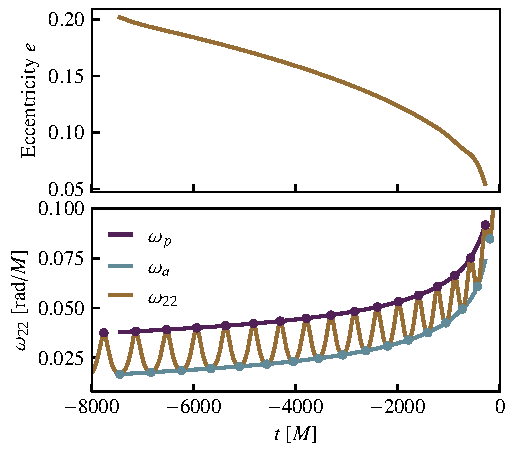
\includegraphics[width=\columnwidth]{ecc_definition} &
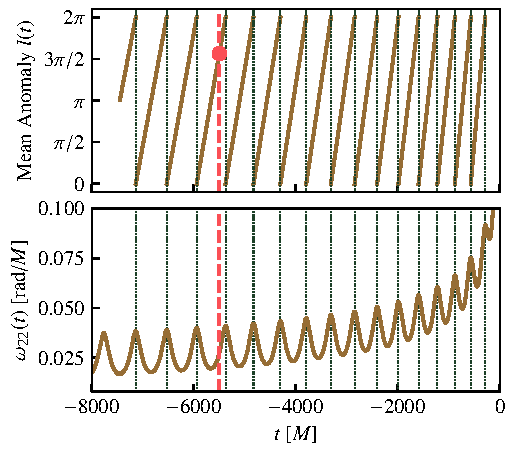
\includegraphics[width=\columnwidth]{mean_ano_definition}
  \end{tabular}
  \caption{{\itshape left:} Time evolution of the eccentricity $e(t)$
(upper panel) and the frequency of (2, 2) mode $\omega_{22}(t)$ (lower
panel) for NR simulation (insert the simulation id here).
$\omega_p(t)$ and $\omega_a(t)$ are spline interpolants of the
frequency of (2, 2) mode at the pericenter and apocenter,
respectively. The spine interpolants $\omega_p(t)$ ad $\omega_a(t)$
are created using the values of $\omega_{22}$ at the pericenter (local
maxima, deep violet circles) and the apocenter (local minima, cyan
circles), respectively. {\itshape right:} Time evolution of the mean
anomaly $l(t)$ (upper panel) and the $\omega_{22}(t)$ (lower
panel). The vertical green dotted lines denote the local maxima (times
of passage of pericenter). The mean anomaly varies linearly with time
between two successive passages of pericenter. The slope of $l(t)$
becomes steeper as the binary inspirals due the reducing radial
period. The red dashed line on all the panels indicates the reference
time $\tref=-5500$ and the red circle on upper left panel and upper
right panel denotes the measured value of the eccentricity and mean
anomaly, respectively, at $\tref$.}
  \label{fig:ecc_definition}
\end{figure*}

%==========================================================================
\section{Implementation}
\label{sec:implementation}
In this section, we discuss different methods and their
implementations in our public \texttt{Python} library (\TODO{what do
  we call it?}) to measure the eccentricity and mean anomaly from
gravitational wave data.

\subsection{Methods to locate pericenter and apocenter}
\label{sec:method-to-locate-pericenter-and-apocenter}
To measure eccentricity using the definition in
eq. (\ref{eq:eccentricity_definition}), the most crucial step is to
locate the positions of pericenters and apocenters from the
gravitational waveform. Below we discuss different ways to accomplish
this and discuss their advantages and disadvantages as well. These
different methods differ mainly in what data they use to
find the locations of the pericenters and the apocenters.

\subsubsection{Frequency and Amplitude}
\label{sec:frequency-and-amplitude}
The most straightforward and perhaps easiest way to locate the positions of the
pericenters and the apocenters is to use the instantaneous
$\omega_{22}(t)$ and find the local maxima in it using a peak finding
routine. For example, in our package, we use a public routine from
\texttt{scipy.signal} called \texttt{find\_peaks} to find the positions
of the local maxima, i. e., the pericenters. We can find the positions
of the local minima, i. e., the apocenters in the same way but just
changing the sign of the $\omega_{22}(t)$ since the
\texttt{find\_peaks} routine is designed to find the local maxima
only. We call this method of find the locations of pericenters and
apocenters using the $\omega_{22}$ data as \mFreq{}.

The next method that we implemented is called \mAmp{} and
as the name suggests it uses the same procedure to locate the
pericenters and apocenters but uses the instantaneous amplitude
$A_{22}$ instead of the $\omega_{22}$.

There is one advantage of using \mAmp{} over using
\mFreq{} specially for numerical relatively waveforms where
often the $\omega_{22}$ data is noisier than the $A_{22}$ data and
therefore it is safer to use the $A_{22}$. Otherwise using noisy
$\omega_{22}$ data may lead to spurious local maxima and minima and
that would in turn give in correct measurement of the eccentricity and
mean anomaly.

However, both the \mFreq{} and \mAmp{} method has the disadvantages
that these methods do not work well for low eccentricities since the
peak finding routines fail to detect the local maxima and minima in
the $\omega_{22}$ and $A_{22}$ data due to the reduced modulations in
them. In fig. \ref{fig:amp_vs_res_amp}, it is seen that the \mAmp{}
method is able to detect only the first few local maxima (shown by violet
circles) and after that it does not pick any local maxima. This
motivates us to consider other ways to detect local maxima and minima
that would work for even low eccentricities where the \mFreq{} and
\mAmp{} method fail.

\begin{figure}[thb]
  \centering
  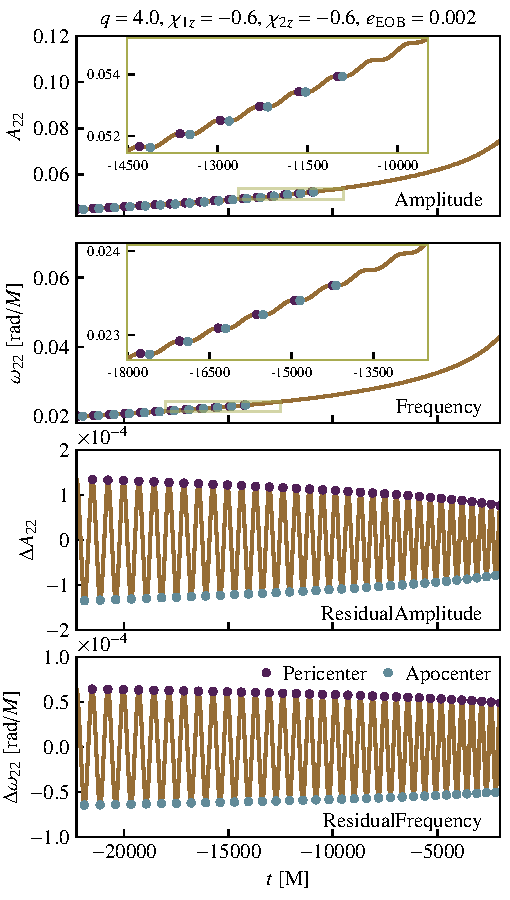
\includegraphics[width=\columnwidth]{compare_methods}
  \caption{Illustration of how well \mAmp{} and \mResAmp{} can detect
the local maxima for a waveform of low eccentricity. The \mAmp{}
method can detect only the very first few maxima (violet circles) and
fails to detect the rest of the maxima. On the other hand, the
\mResAmp{} method can detect all the local maxima (red circles) in the
$\omega_{22}(t)$ (brown solid line).}
  \label{fig:amp_vs_res_amp}
\end{figure}

\subsubsection{Residual frequency and residual amplitude}
\label{sec:residual-frequency-and-residual-amplitude}
As the eccentricity becomes smaller the modulations in $\omega_{22}$
and $A_{22}$ becomes smaller and we want to find a way to detect these
small modulations to locate the local maxima and minima in them. One
way to do this is to substract some sort of average of the
instantaneous $\omega_{22}(t)$ from the instantaneous $\omega_{22}(t)$
itself and get a residual $\resOmega$. It is observed that for any
eccentric waveform the instantaneous $\zeroOmega(t)$ of corresponding
quasi-circular waveform (that has all the binary parameters the same
except that the eccentricity is zero) can act as such an average
$\omega_{22}$. Fig. \ref{fig:eccentric-and-non-eccentric}, the upper
panel shows amplitude $A_{22}$ for an eccentric EOB waveform (solid
line) and a quasi-circular waveform (dashed line) aligned at the
merger. The lower panel shows the same for the $\omega_{22}$. 

\begin{figure}[htb]
  \centering
  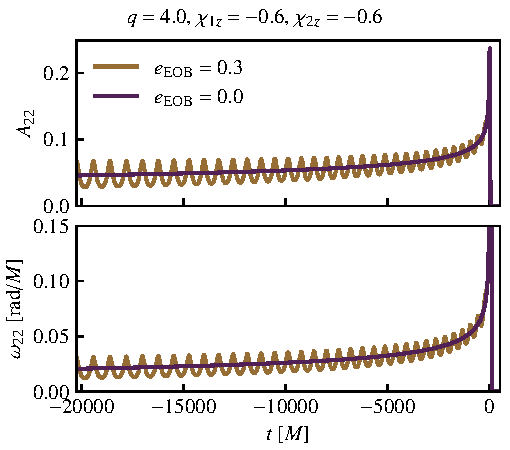
\includegraphics[width=\columnwidth]{ecc_and_zero_ecc}
  \caption{eccentric and quasi-circular amplitude and frequency}
  \label{fig:eccentric-and-non-eccentric}
\end{figure}

Thus, we can construct a residual
frequency $\resOmega$ by aligning the waveforms at the merger
and then substracting the $\omega_{22}(t)$ of the quasi-circular
waveform from the $\zeroOmega(t)$ of the eccentric waveform.
\begin{equation}
  \label{eq:residual-omega22}
  \resOmega(t) = \omega_{22}(t) - \zeroOmega(t)
\end{equation}

We then follow the same steps as discussed in
sec. \ref{sec:frequency-and-amplitude} but use $\resOmega(t)$
instead of $\omega_{22}(t)$ to find the local maxima and minima. We
call this method \mResFreq{}.

Similarly one can construct a residual amplitude $\resAmp$ by
substracting the quasi-circular amplitude $\zeroA$ from
eccentric amplitude $A_{22}$

\begin{equation}
  \label{eq:residual-amplitude}
  \resAmp(t) = A_{22}(t) - \zeroA(t)
\end{equation}

\mResAmp{} method uses the residual amplitude $\Delta
A_{22}$ to find the local maxima and minima.

The advantage of the residual methods is that these methods can detect
the locations of local maxima and minima accurately even for very
small eccentricities. In fig. \ref{fig:amp_vs_res_amp}, it could be
seen that the \mResAmp{} method (red circles) can detect all the local
maxima that the \mAmp{} method (violet circles) was unable to
detect. The disadvantage of the residual methods is that they need a
corresponding quasi-circular waveform. (\TODO{EXPAND and IMPROVE
this})

\subsubsection{Frequency fits}
\label{sec:frequenc-fits}

\TODO{Harald should fill this in.}

\subsection{Defining $\avgOmega(t)$}
\label{sec:definig-average-omega22}

To measure the eccentricity and mean anomaly at a reference frequency $\fref$
we need a $\avgOmega$ so that we can get the reference
time $\tref$ using
eq. (\ref{eq:map-between-ref-freq-and-ref-time}). Below we discuss
different ways of implementing such an $\avgOmega$

\subsubsection{Orbital average at the extrema}
\label{sec:orbital-average-at-the-extrema}
In this implementation, we get the orbital average of the
$\omega_{22}(t)$ at the extrema. At the $i$th extrema the
$\avgOmega[t_i]$ is computed as

\begin{equation}
  \label{eq:orbital-average-at-extrema}
  \avgOmega[t_i] = \frac{1}{t_{i+1} -
    t_{i}}\int_{t_{i}}^{t_{i+1}}\omega_{22}(t) dt,
\end{equation}
where $t_{i+1}$ is the time of the $i+1$th extrema. We associate this
$\avgOmega[t_{i}]$ with the time $t = (t_i +
t_{i+1})/2$. Once we get the orbital average of $\omega_{22}(t)$ at
all the extrema using eq. (\ref{eq:orbital-average-at-extrema}), we
create an interpolant $\avgOmega(t)$.

\subsubsection{Average between the extrema}
\label{sec:average-between-the-extrema}
For the eccentricity measurement we create the interpolants
$\omega_{p}(t)$ and $\omega_a(t)$ which uses the $\omega_{22}$ values
at the pericenter and the apocenters, respectively. This
implementation of $\avgOmega$ uses these two
interpolants and takes the mean of these
\begin{equation}
  \label{eq:average-between-extrema}
  \avgOmega(t) = \frac{\omega_{p}(t) + \omega_{a}(t)}{2}.
\end{equation}

\subsubsection{Quasi-circular frequency}
\label{sec:quasi-circular-frequency}
Another option to get the $\avgOmega$ is to just use
the $\zeroOmega$ of the corresponding quasi-circular waveforms
where the quasi-circular waveform is generated using the same set of
binary parameters as the eccentric one except that for the
quasi-circular waveform, the eccentricity $e$ is set to zero. Thus we
can use
\begin{equation}
  \label{eq:quasi-circular-frequency}
  \avgOmega(t) = \zeroOmega(t).
\end{equation}

Fig. \ref{fig:omega22-average}, $\avgOmega$ is shown for different
averaging methods.

\begin{figure}[htb]
  \centering
  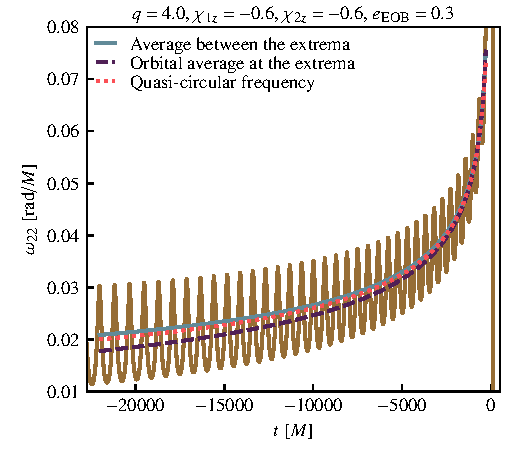
\includegraphics[width=\columnwidth]{omega22_average}
  \caption{omega22 average}
  \label{fig:omega22-average}
\end{figure}
% ==========================================================================

\section{Demonstrations}
\label{sec:demonstrations}
\begin{figure*}[htb]
  \centering
  \begin{tabular}{cc}
    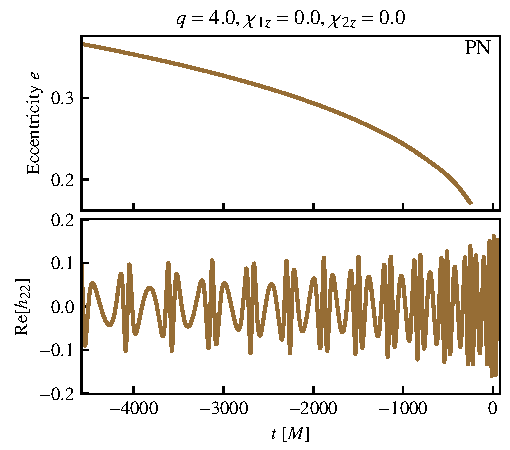
\includegraphics[width=\columnwidth]{demo_PN} & 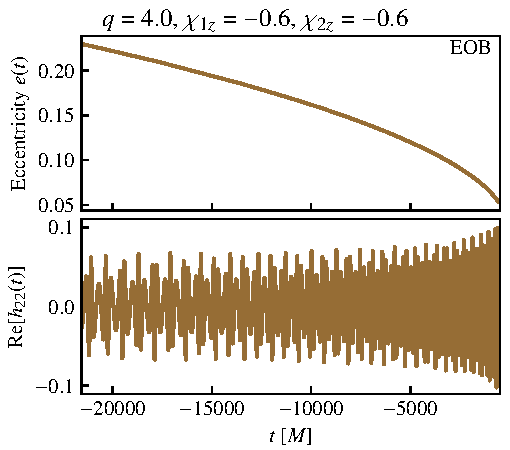
\includegraphics[width=\columnwidth]{demo_EOB}\\
     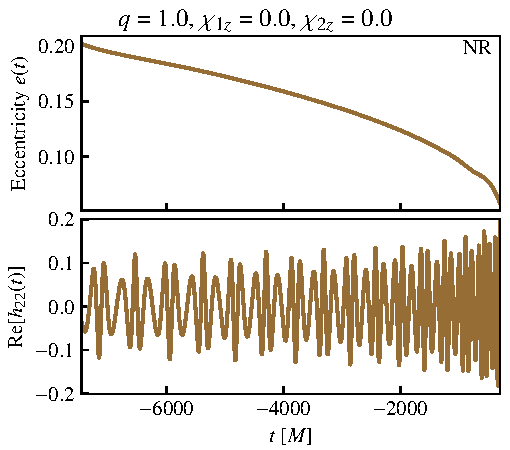
\includegraphics[width=\columnwidth]{demo_NR} &
  \end{tabular}
  \caption{Demo of measuring eccentricity for different waveforms}
  \label{fig:demonstrations}
\end{figure*}



%==========================================================================
\section{Tests of robustness}
\label{sec:tests}
To check the robustness of the eccentricity definition in
(\ref{eq:eccentricity_definition}) and the implementations using
different methods discussed in sec. \ref{sec:implementation}, we put
our implementations through different tests. One of the checks for
robustness of our implementation is to see how well it works for
waveforms of eccentricities varying from very low to high values. For
this purpose, we generate hundreds of EOB waveforms using
\texttt{SEOBNRv4EHM} model (\TODO{cite Toni's paper}) with
eccentricity (this is the eccentricity that the model takes as an
input, we call this EOB eccentricity $\eEOB$) from
$\eEOB = 10^{-7}$ to $\eEOB = 1.0$ keeping other
parameters (mass ratio and spins of the black holes) fixed. We do the
following two tests using these waveforms

\subsection{EOB eccentricity vs measured eccentricity}
\label{sec:eob-eccentricity-vs-measured-eccentricity} In this test, we
compare the eccentricity that the EOB model takes as an input (the EOB
eccentricity $\eEOB$) and the eccentricity that we measure
using our definition in (\ref{eq:eccentricity_definition}) at a
specific reference time. For this test, we choose our reference time
to be at the first available local extremum (pericenter or
apocenter). As we vary the $\eEOB$ smoothly from low to high
values we expect the measured eccentricities to also vary smoothly.
This test also checks whether a particular implementation is able to
measure the eccentricity at all. This is because, as $\eEOB$
becomes smaller and smaller some of the implementations may fail to
detect any local extrema and therefore can not measure eccentricity
beyond a certain $\eEOB$.

Fig. \ref{fig:eob_vs_measured_ecc}, shows how the measured
eccentricities $e$ varies with the EOB eccentricities $\eEOB$ for
waveforms with $q=4, \chi_{1z}=-0.6, \chi_{2z}=-0.6$. It illustrates
robustness of different methods to measure eccentricities from very
low to high $\eEOB$. \mFreq{} and \mResFreq{} is not shown as they
perform similar to \mAmp{} and \mResAmp{}, respectively.  While each
method works nicely for relatively high eccentricities $\eEOB \gtrsim
10^{-2}$, \mAmp{} (solid line) starts to deviate from others and fails
to measure eccentricities as $\eEOB$ becomes close to $10^{-3}$. On
the other hand, \mResAmp{} (dashed line) can measure eccentricities up
to $\eEOB \simeq 10^{-5}$ and after that the measured eccentricities
tend to saturate. \mFreqFits{} (dotted line) works upto
$10^{-4}$. This test implies that while the \mFreq{} and the \mAmp{}
methods work for relatively high eccentricities, they fail to
accurately measure eccentricity or fail to measure eccentricity at all
for low eccentricities. However, the residual methods work and can
accurately measure eccentricity even for very low eccentricities.

%--------------------------------------------------------------------------
\begin{figure}[thb]
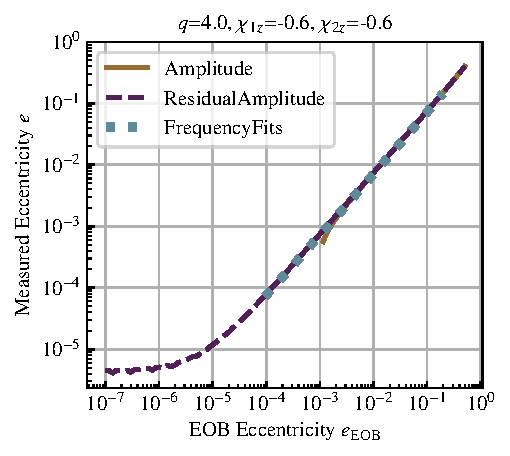
\includegraphics[width=\columnwidth]{test_eob_vs_measured_ecc_example}
\caption{
  EOB eccentricity vs measured eccentricity plots to illustrate the
robustness of different methods to measure eccentricities from very
low to high $\eEOB$. \mFreq{} and \mResFreq{} is not shown as they
perform similar to \mAmp{} and \mResAmp{}, respectively.  While each
method works nicely for relatively high eccentricities $\eEOB \gtrsim
10^{-2}$, \mAmp{} (solid line) starts to deviate from others and fails
to measure eccentricities as $\eEOB$ becomes close to $10^{-3}$. On
the other hand, \mResAmp{} (dashed line) can measure eccentricities up
to $\eEOB \simeq 10^{-5}$ and after that the measured eccentricities
tend to saturate. \mFreqFits{} (dotted line) works upto $10^{-4}$.
}
\label{fig:eob_vs_measured_ecc}
\end{figure}

\subsection{Measured eccentricity vs time}
\label{sec:measured-eccentricity-vs-time}
In this test, we check how the evolution of measured eccentricity with
time vary as we vary the EOB eccentricities for a given method. To
make the visualization better, we color the measured eccentricity vs
time plots as a function of the $\eEOB$ and use a smoothly
varying color gradient to choose the colors from. If a particular
method works for all $\eEOB$ from $10^{-7}$ to $1.0$ and for
all the times upto the merger, then we expect the measured
eccentricity vs time plots for that method to form a band of colors
smoothly varying from color of one end to the other end of the color
gradient we are using. We also expect each line representing the
evolution of measured eccentricity to be smooth and monotonically
decreasing.

Fig. \ref{fig:measured_ecc_vs_time} the results of this test. The text
at the top right corner of each panel indicate the method that was
used to measure the eccentricity of the EOB waveforms starting with
eccentricity $\eEOB$. The \mAmp{} and the
\mFreq{} methods work well upto $\eEOB \simeq
10^{-2}$ and below that the $e(t)$ curves stop further and further
away from the merger and finally fail to measure any eccentricity. On
ther other hand, the \mResAmp{} and
\mResFreq{} methods work well upto $\eEOB
\simeq 10^{-5}$ and the $e(t)$ curves go all the way up to the
merger.

There are sudden jumps and the glitches, noticable in
particular for low $\eEOB$s, in the evolution of the measured
eccentricities for the two residual methods.  This is due to the jump
and glitches in $\omega_{22}$ data of the EOB waveform itself and not
a drawback of the methods. In fig. \ref{fig:res-amp-glitches}, we
explain these jumps in the eccentricity evolution using one EOB
waveform with $q=4.0, \chi_{1z}=-0.6, \chi_{2z}=-0.6$ and $\eEOB=1.07
\into 10^{-5}$ at initial $\omega_{22} = 0.01$. In the upper panel,
there is a big jump in
the $e(t)$ curve around $t=-10000$ which is indicated by a red dashed
line. In the lower panel, $\resOmega$ is plotted as a function of time
and it is indeed seen that apocenters (cyan circles) and pericenters
(violet circles) accurately correspond to the extrema of the
$\resOmega$ and at around $t=10000$, there is a jump in the
$\resOmega$ values at the extrema which corresponds to the jump in the
$e(t)$ curve in the upper panel.

\begin{figure}[thb]
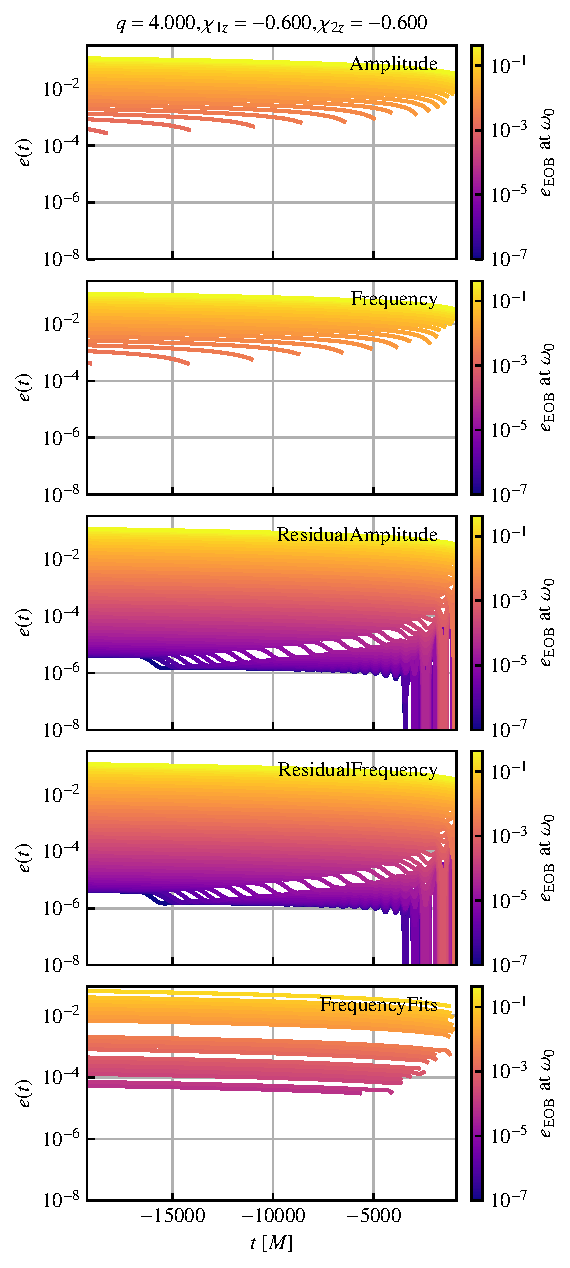
\includegraphics[width=\columnwidth]{test_measured_ecc_vs_time_example}
\caption{
  Evolution of $e(t)$ (measured eccentricity) for varying $\eEOB$ (EOB
eccentricity). Text at top right corner indicates the used method. The
colorbar on right indicates the $\eEOB$ of the waveforms
used. \mAmp{} and \mFreq{} methods work well upto
$\eEOB \simeq 10^{-2}$ and below that the evolution stops further and
further away from the merger. \mResAmp{} and
\mResFreq{} methods work well upto $\eEOB \simeq
10^{-5}$ and the evolution goes all the way up to the merger. Refer to
the text for more details.
}
\label{fig:measured_ecc_vs_time}
\end{figure}

\begin{figure}[thb]
  \centering
  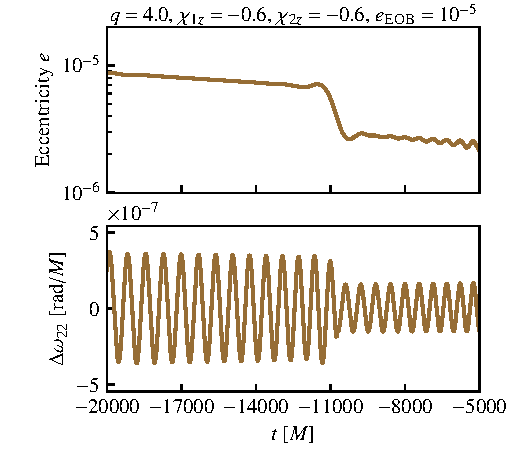
\includegraphics[width=\columnwidth]{res_amp_glitches}
  \caption{Eccentricity evolution using EOB waveform with $q=4.0,
\chi_{1z}=-0.6, \chi_{2z}=-0.6$ and $\eEOB=1.07 \into 10^{-5}$ at
initial $\omega_{22} = 0.01$. In the upper panel, there is a big jump
in the $e(t)$ curve around $t=-10000$ which is indicated by a red
dashed line. In the lower panel, $\resOmega$ is plotted as a function
of time and it is indeed seen that apocenters (cyan circles) and
pericenters (violet circles) accurately correspond to the extrema of
the $\resOmega$ and at around $t=10000$, there is a jump in the
$\resOmega$ values at the extrema which corresponds to the jump in the
$e(t)$ curve in the upper panel.}
  \label{fig:res-amp-glitches}
\end{figure}

%==========================================================================
\section{Conclusion}
\label{sec:conclusion}
Here's what you should learn now that I done'd it.


%==========================================================================
\begin{acknowledgments}
% Randos
We thank Bob Loblaw for useful discussions.
% M.A.S
M.A.S.’s research was supported by the Department of Atomic Energy,
Government of India. M.A.S acknowledges travel support from Infosys
Exchange Scholars program to visit AEI, Potsdam and hospitality by
AEI, Potsdam where a significant part of the work was accomplished.
% V.V
V.V acknowledges support from the European Union’s Horizon 2020
research and innovation program under the Marie Skłodowska-Curie grant
agreement No.~896869.
% LIGO
This material is based upon work supported by NSF's LIGO Laboratory
which is a major facility fully funded by the NSF.
% GWOSC
%This research made use of data, software and/or web tools obtained from the
%Gravitational Wave Open Science Center~\cite{GW_open_science_center}, a service
%of the LIGO Laboratory, the LIGO Scientific Collaboration and the Virgo
%Collaboration.
\end{acknowledgments}

%%%%%%%%%%%%%%%%%%%%%%%%%%%%%%%%%%%%%%%%%%%%%%%%%%%%%%%%%%%%%%%%%%%%%%%%%%%%%%%
\section*{References}
%%%%%%%%%%%%%%%%%%%%%%%%%%%%%%%%%%%%%%%%%%%%%%%%%%%%%%%%%%%%%%%%%%%%%%%%%%%%%%%
\bibliography{References}


\end{document}
